\section{Выполнение}
\subsection{Данные процессора}
% TODO: \usepackage{graphicx} required
\begin{figure}
	\centering
	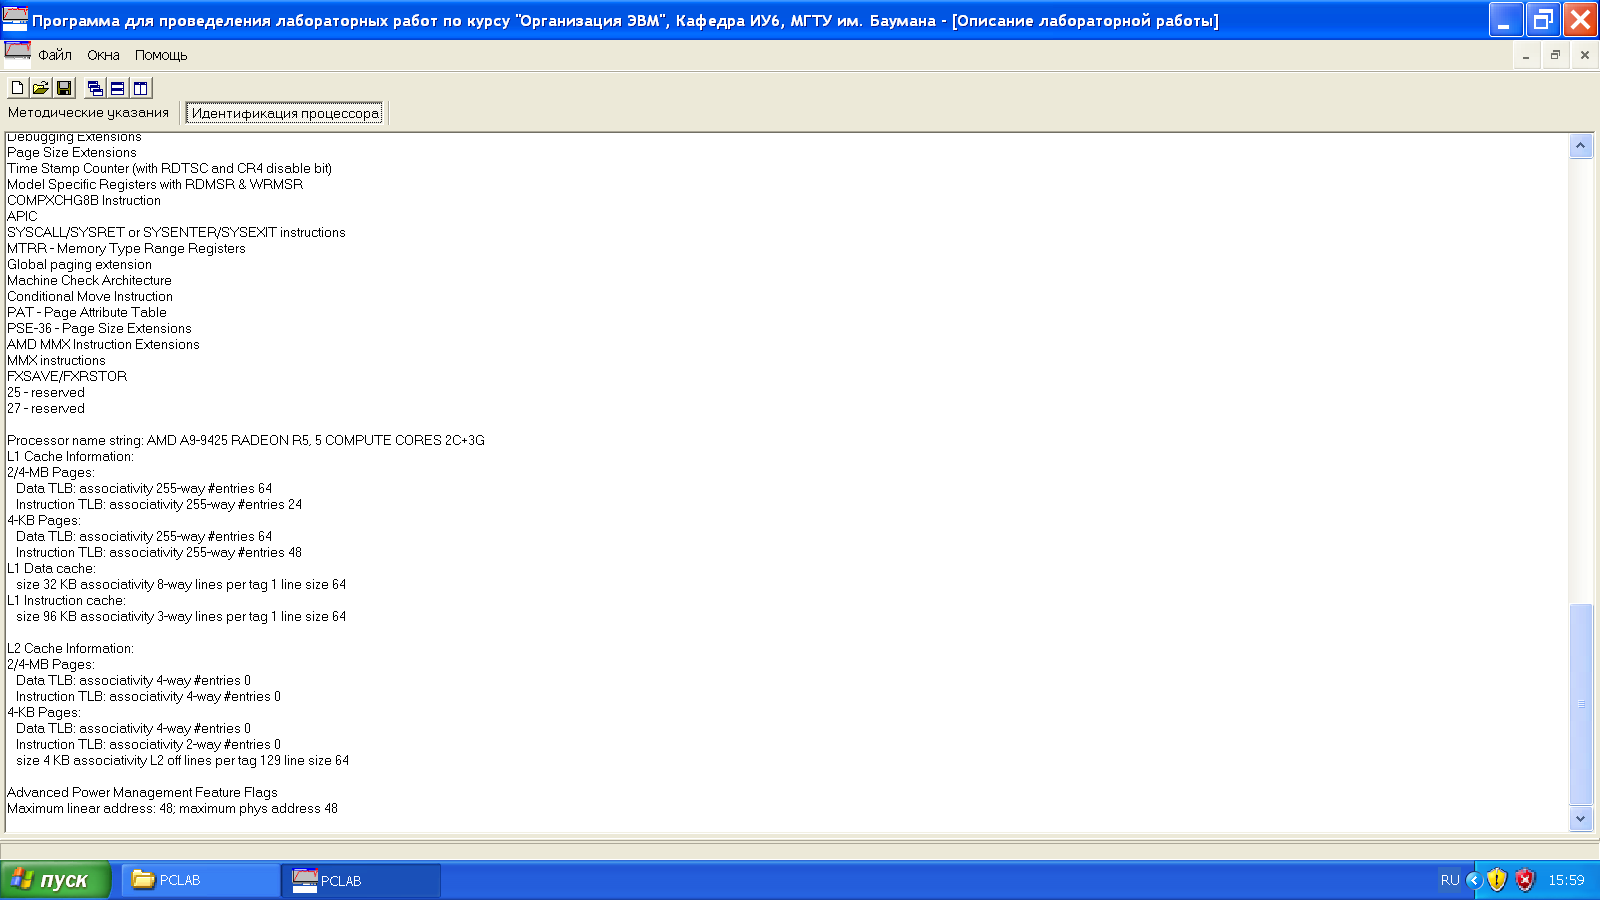
\includegraphics[width=1\linewidth]{../images/screenshot001}
	\caption{данные процессора (часть 1)}
	\label{fig:screenshot001}
\end{figure}
% TODO: \usepackage{graphicx} required
\begin{figure}
	\centering
	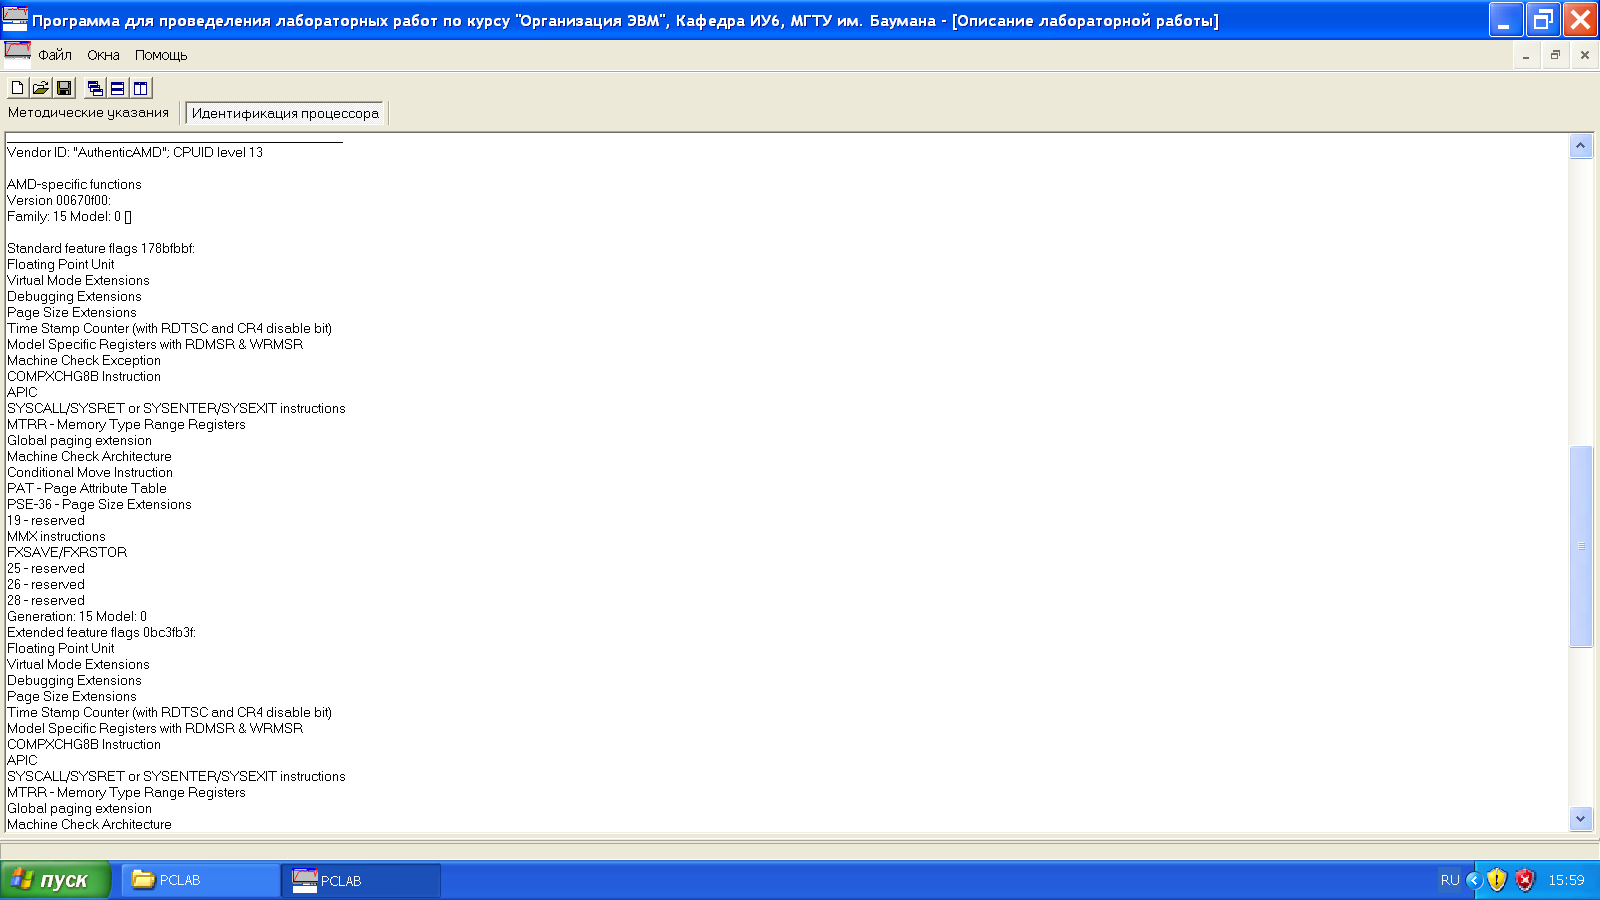
\includegraphics[width=1\linewidth]{../images/screenshot002}
	\caption{данные процессора (часть 2)}
	\label{fig:screenshot002}
\end{figure}
\subsection{Лабораторные работы}
% TODO: \usepackage{graphicx} required
\begin{figure}
	\centering
	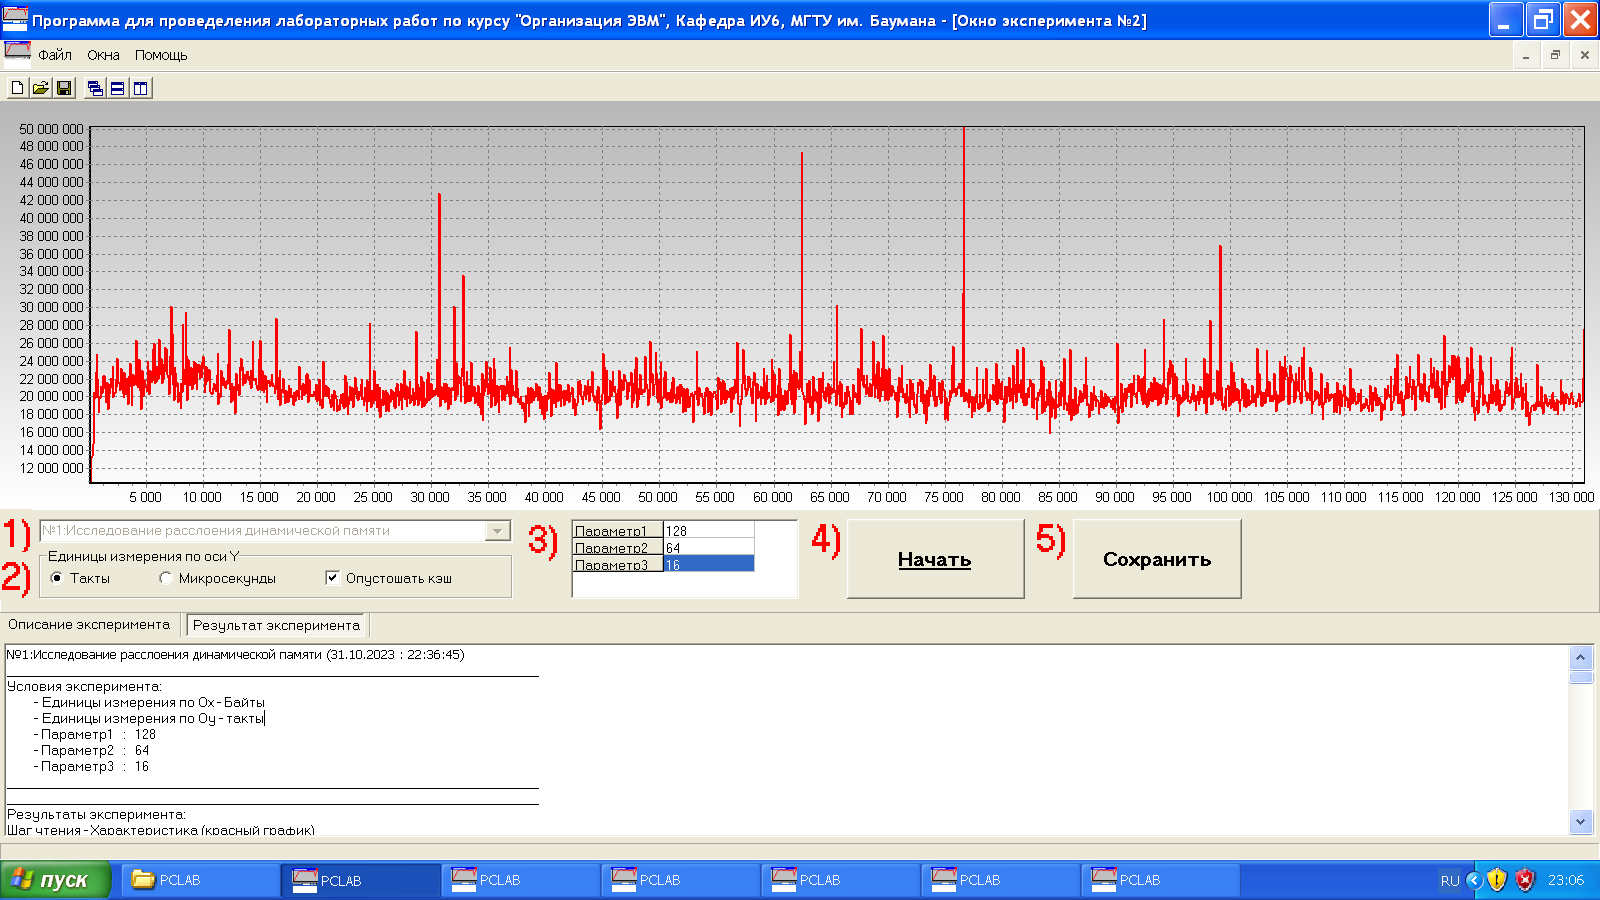
\includegraphics[width=1\linewidth]{../images/screenshot003}
	\caption{результат выполнения ЛР№1}
	\label{fig:screenshot003}
\end{figure}
% TODO: \usepackage{graphicx} required
\begin{figure}
	\centering
	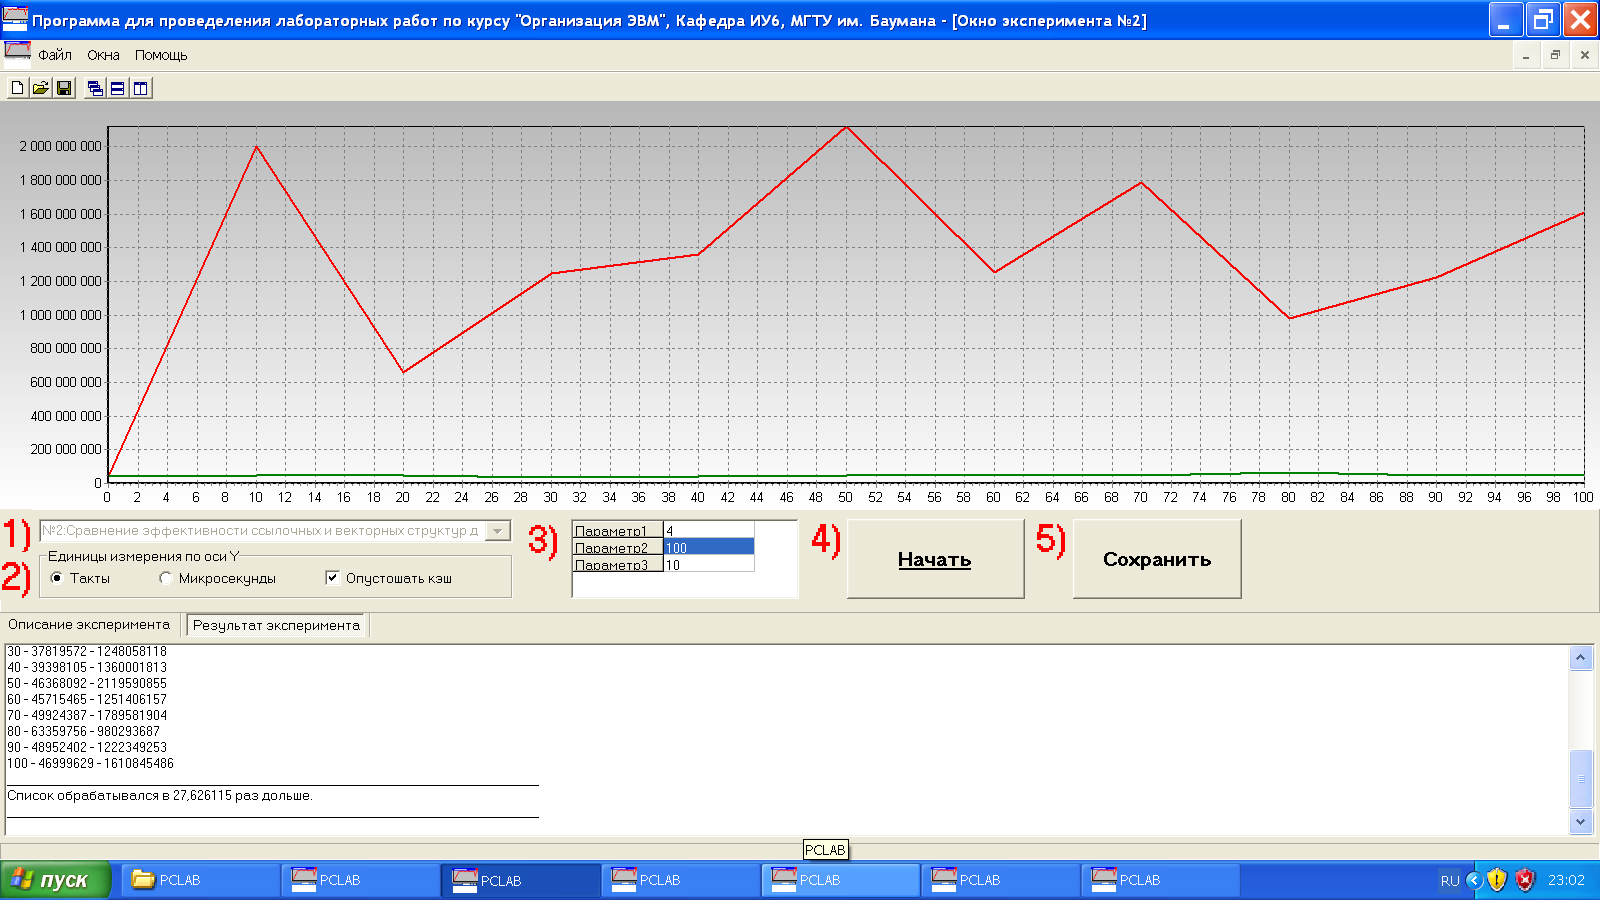
\includegraphics[width=1\linewidth]{../images/screenshot004}
	\caption{результат выполнения ЛР№2}
	\label{fig:screenshot004}
\end{figure}
% TODO: \usepackage{graphicx} required
\begin{figure}
	\centering
	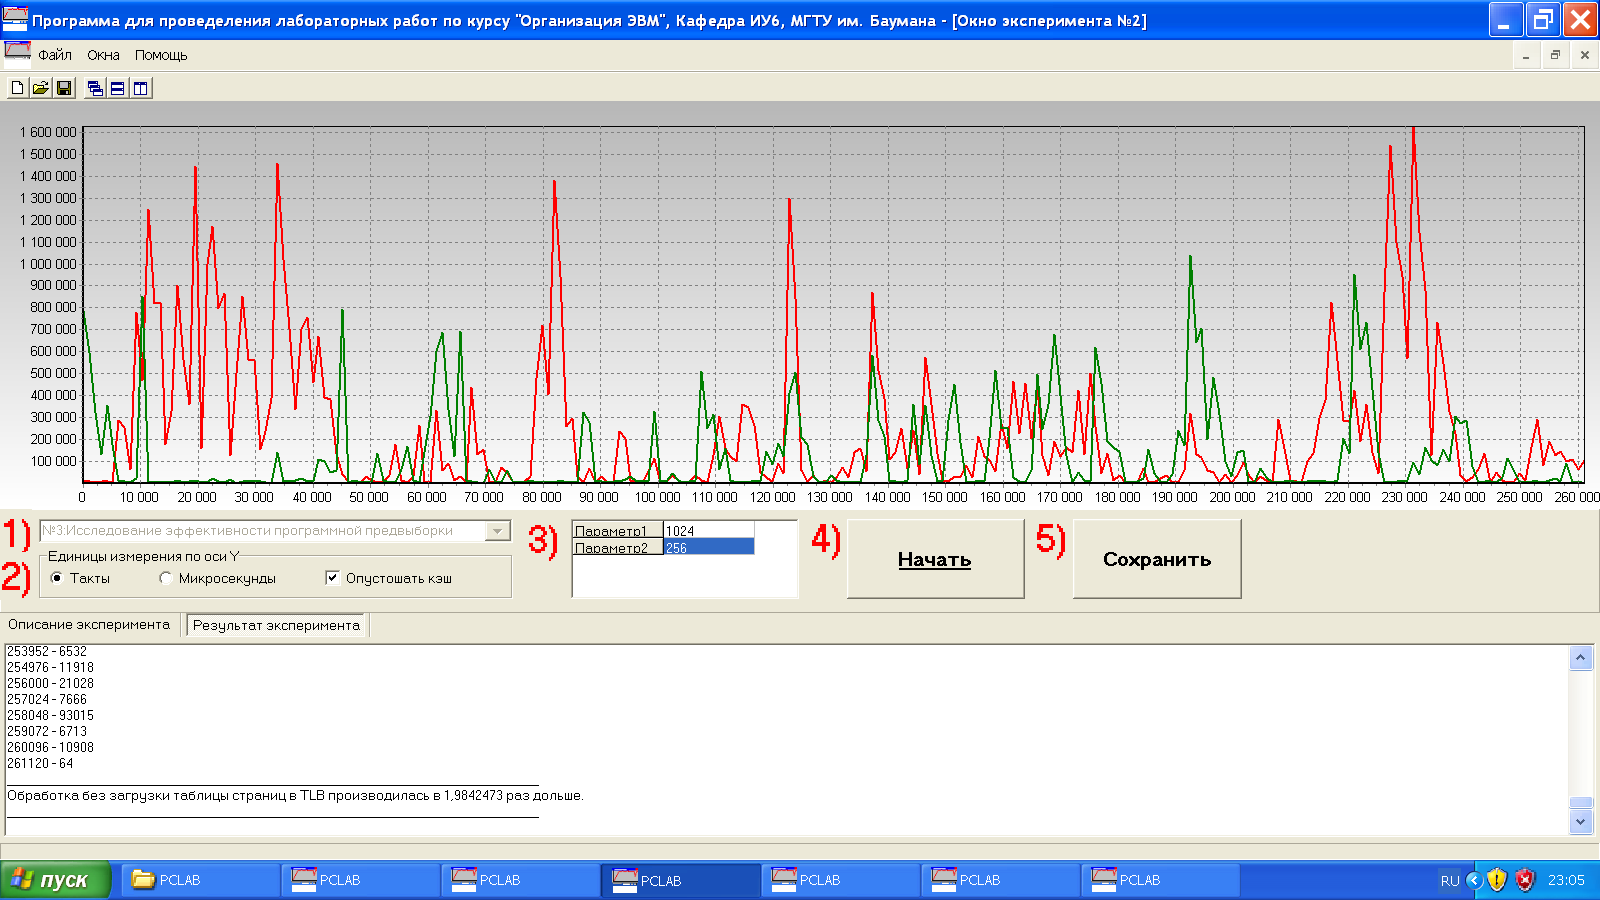
\includegraphics[width=1\linewidth]{../images/screenshot005}
	\caption{результат выполнения ЛР№3}
	\label{fig:screenshot005}
\end{figure}
% TODO: \usepackage{graphicx} required
\begin{figure}
	\centering
	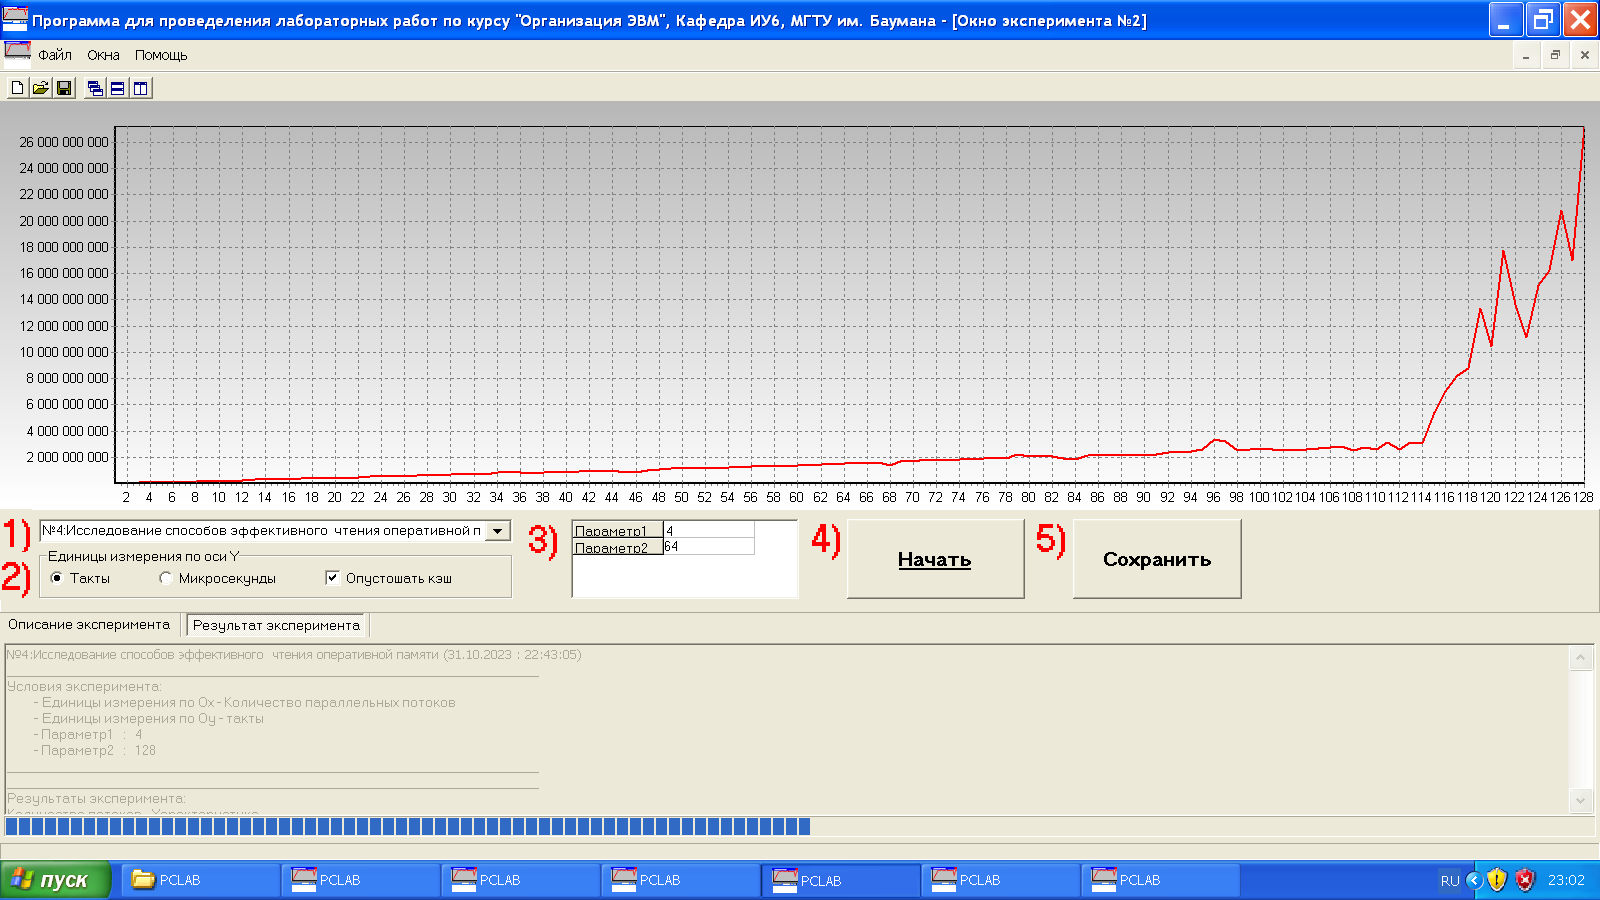
\includegraphics[width=1\linewidth]{../images/screenshot009}
	\caption{результат выполнения ЛР№4}
	\label{fig:screenshot009}
\end{figure}
% TODO: \usepackage{graphicx} required
\begin{figure}
	\centering
	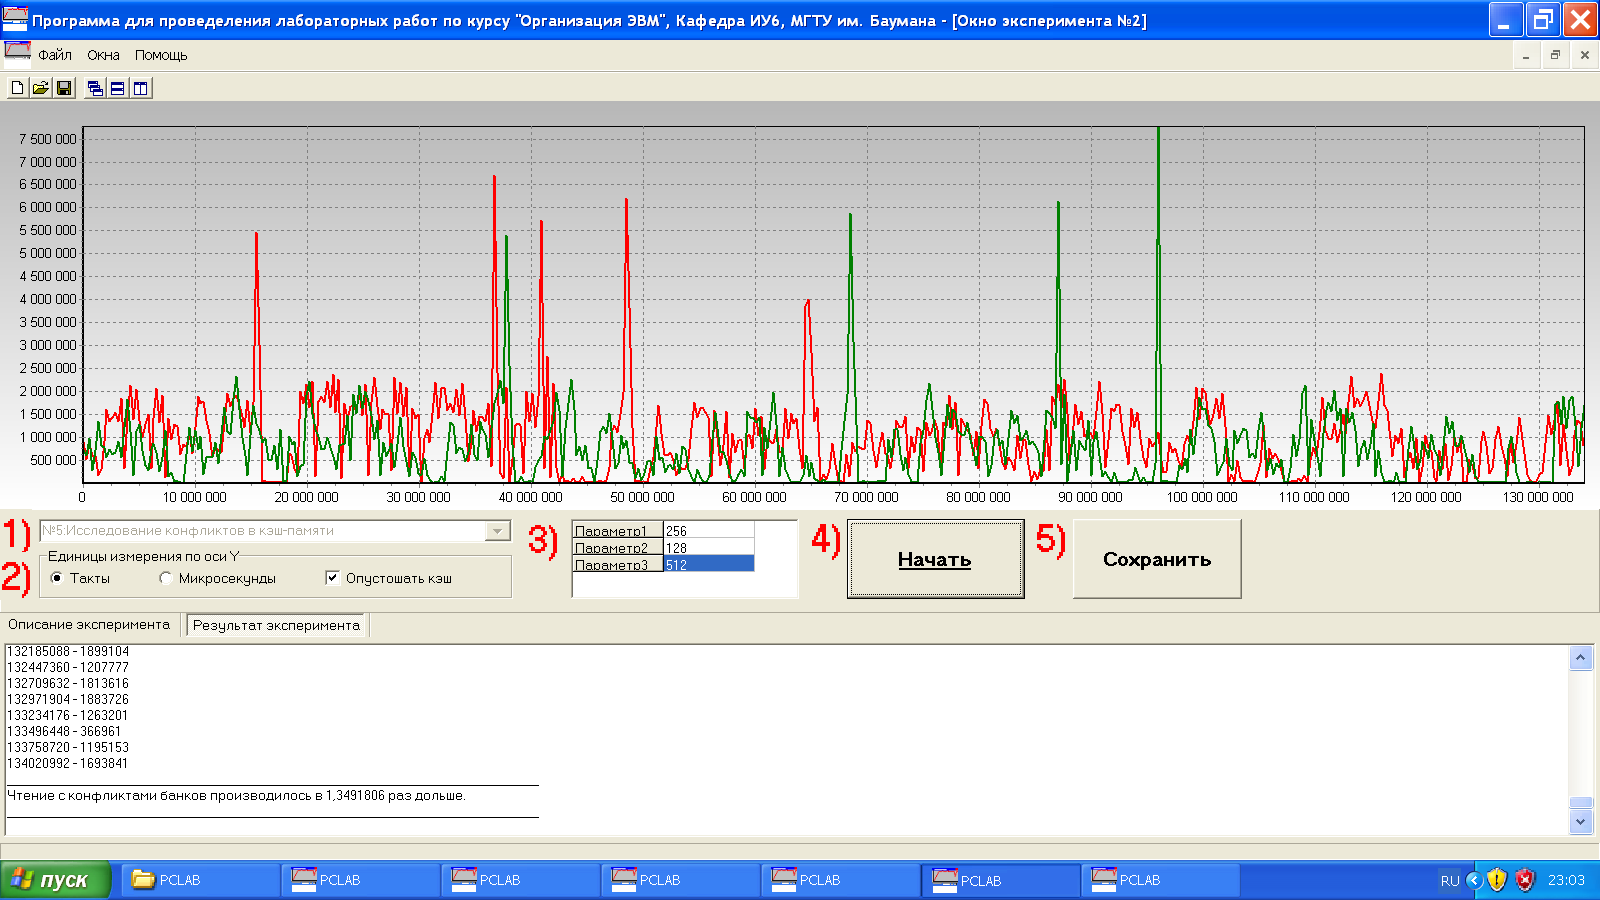
\includegraphics[width=1\linewidth]{../images/screenshot007}
	\caption{результат выполнения ЛР№5}
	\label{fig:screenshot007}
\end{figure}
% TODO: \usepackage{graphicx} required
\begin{figure}
	\centering
	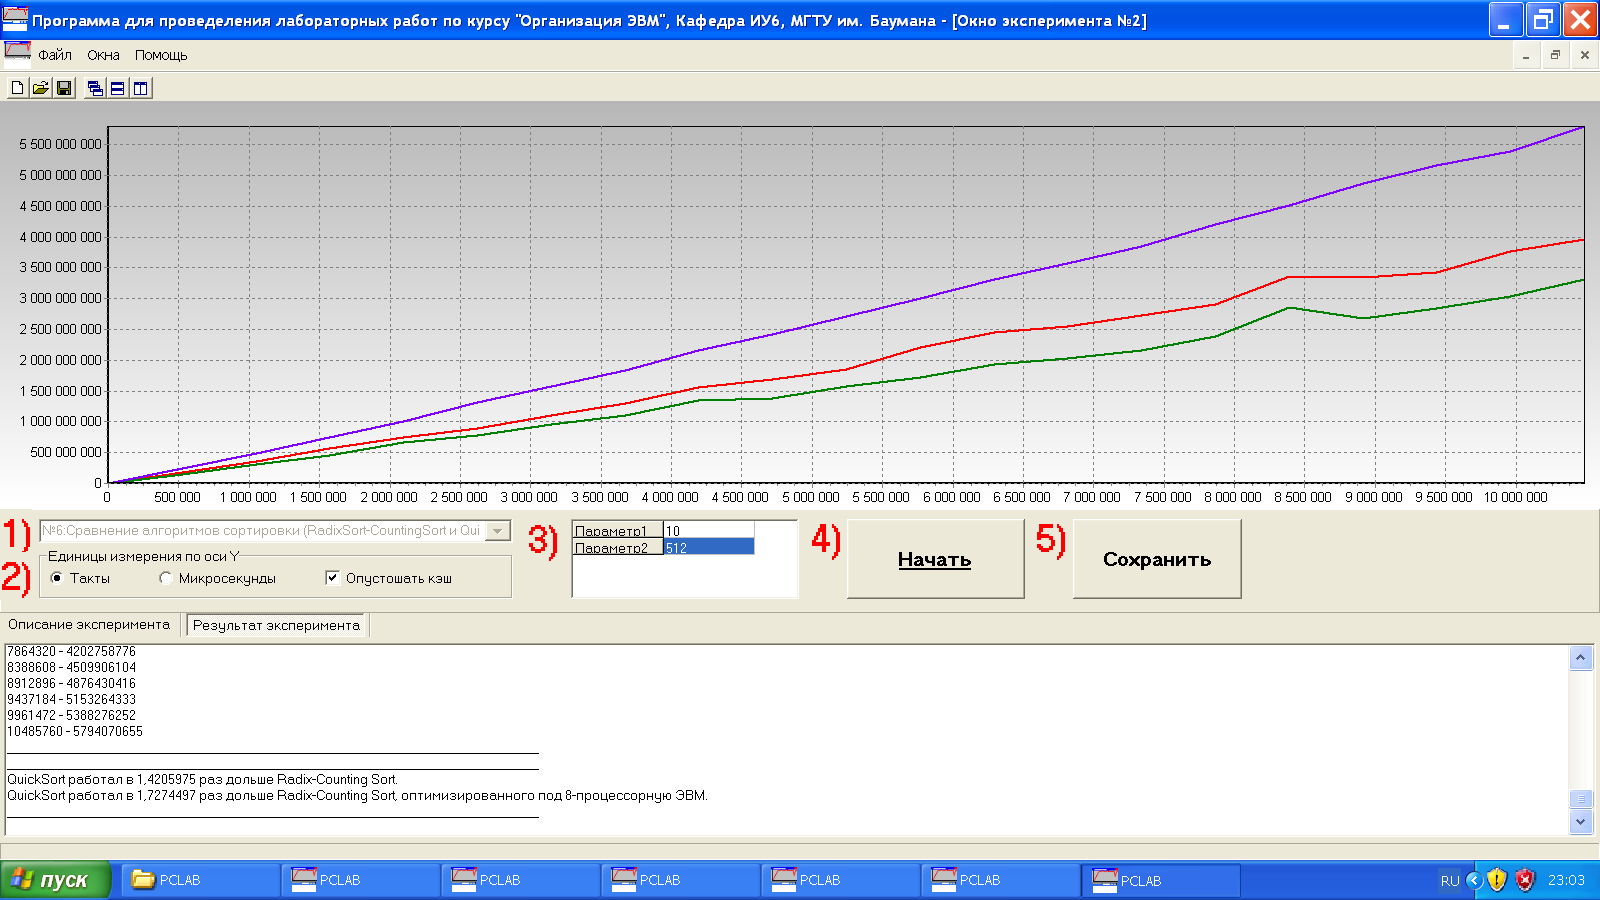
\includegraphics[width=1\linewidth]{../images/screenshot008}
	\caption{результат выполнения ЛР№6}
	\label{fig:screenshot008}
\end{figure}

